\documentclass[12pt,a4paper]{article}
\usepackage[utf8]{inputenc}
\usepackage[english]{babel}
\usepackage{amsmath}
\usepackage{amsfonts}
\usepackage{amssymb}
\usepackage{graphicx}
\graphicspath{ {./graphics/} }

\usepackage[top=1.5in, bottom=1in, left=1in, right=1in]{geometry}

\usepackage{hyperref}

\usepackage{float}

\usepackage{subcaption}

\usepackage{tikz}
\usetikzlibrary{arrows,automata, positioning,calc,shapes.geometric}

% header
\usepackage{fancyhdr}
\pagestyle{fancyplain}
\fancyhf{}
\lhead{ \fancyplain{}{Lukas Schwartz \& Aitor Miguel } }
\rhead{ \fancyplain{}{AI1 - 1. Semester MSc Robot Systems} }
\cfoot{ \fancyplain{}{\thepage} }

% make tables prettyer
\def\arraystretch{1.3}

\usepackage{todonotes}

\begin{document}

\begin{titlepage}
	\centering
%	\includegraphics[width=0.15\textwidth]{example-image-1x1}\par\vspace{1cm}
	\vfill
	{\scshape\LARGE University of Southern Denmark\par}
	\vspace{1cm}
	{\scshape\Large AI1 Project \#1\par}
	{\scshape\large 1. Semester MSc Robot Systems\par}
	\vspace{1.5cm}
	{\huge\bfseries Sokoban Solver\par}
	\vspace{2cm}
	{\Large\itshape Aitor Miguel Blanco \& Lukas Chr. M. W. Schwartz \\ Group \#1 \par}
	\vfill
	supervised by\par
	John Hallam

	\vspace{2cm}

% Bottom of the page
	{\large 18$^{th}$ December 2015 \par}
\end{titlepage}

\pagebreak

\tableofcontents

\pagebreak

\listoffigures

\listoftables

\pagebreak

\section{Introduction}

In this project, the problem of solving automatically the sokoban game has been faced.
To do this, the project has been divided in two different parts, being studied separately.
These are finding the shortest solution given a sokoban map and the hardware implementation of a robot able to execute the generated path.

The system loads a map and finds a solution offline with a solver. 
The output of this program is a path that the robot should follow. 
This path is loaded onto the robot, which is prepared to execute it on the sokoban map.

The robot designed is made using different LEGO and LEGO Mindstorms parts and an NXT as controller.
And the solver is programmed using C++.

%The solver is based in the A* algorithm and implemented in C++.

\pagebreak
\section{Robot Design}
To solve the sokoban problem a robot capable of performing simple tasks concerned with moving the can and itself around the game map are needed.
The behaviours the robot should be able to perform define how the robot should be formed in order to accomplish its task of solving the sokoban problem.

\subsection{System Behaviours}
The robot was decided to be build upon being able to execute simple behaviours.
The execution of the behaviours would then be controlled from the \textit{Brain},
this is illustrated in figure \ref{fig:behaviourSystem}.

% brain/behaviour diagram
\begin{figure}[H]
\center
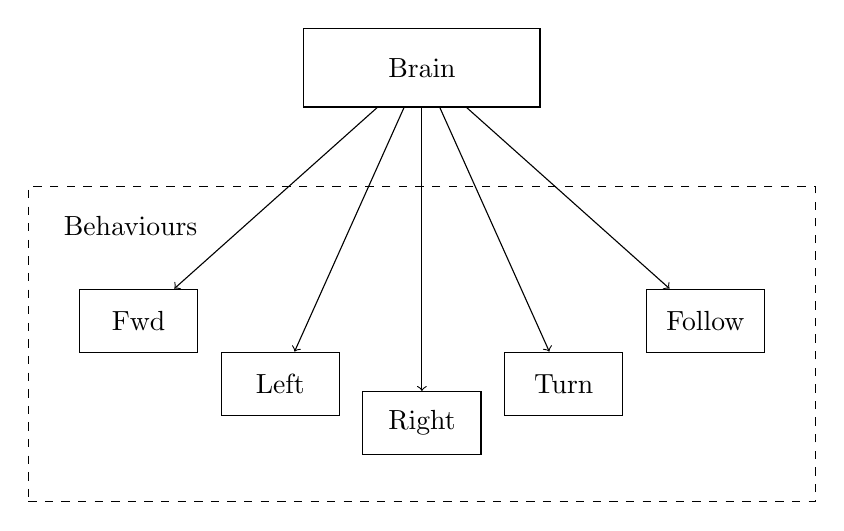
\begin{tikzpicture}[node distance=1cm]
%  behaviour box
\node[rectangle,draw,minimum width=10cm, minimum height=4cm, dashed, name=behaviour_box]  at (0,0) {};
\node[name=behaviour] at (-3.7,1.5) {Behaviours};

% Brain node 
\node[rectangle,draw,minimum width=3cm, minimum height=1cm, name=brain, above=of behaviour_box] {Brain};

% behaviours
\node[rectangle,draw,minimum width=1.5cm, minimum height=0.8cm, name=fwd] at (-3.6,0.3) {Fwd};
\node[rectangle,draw,minimum width=1.5cm, minimum height=0.8cm, name=left] at (-1.8,-0.5) {Left};
\node[rectangle,draw,minimum width=1.5cm, minimum height=0.8cm, name=right] at (0,-1.) {Right};
\node[rectangle,draw,minimum width=1.5cm, minimum height=0.8cm, name=turn] at (1.8,-0.5) {Turn};
\node[rectangle,draw,minimum width=1.5cm, minimum height=0.8cm, name=follow] at (3.6,0.3) {Follow};

% arrows inside 
\draw[->] (brain) -- (fwd) ;
\draw[->] (brain) -- (left) ;
\draw[->] (brain) -- (right) ;
\draw[->] (brain) -- (follow) ;
\draw[->] (brain) -- (turn) ;
\end{tikzpicture}
\caption{Overview of the systems behaviours.}
\label{fig:behaviourSystem}
\end{figure}

Here the central unit, the \textit{Brain} is responsible for finding the solution to the sokoban problem by invoking the five behaviours.
The \textit{Brain} is hence a combination of both the computer processing the map offline and the Lego-robot online when using the offline generated data to solve the puzzle.

The behaviours are defined in table \ref{tab:behaviourExplained} and based on dividing the behaviours into simple tasks which are easy to program.

\begin{table}[H]
\center
\begin{tabular}{c|l}
Behaviour & Description \\ \hline
Fwd & Makes the robot go straight ahead in the next intersection. \\
Left / Right & The robot turns left/right in the next intersection. \\
Turn & Turns the robot 180 degrees around in the next intersection. \\
Follow & Makes the robot follow the line till next intersection.
\end{tabular}
\caption{Behaviour table.}
\label{tab:behaviourExplained}
\end{table}

\todo[inline]{what about a separate push behaviour?}

With these five behaviours the robot should then be able to navigate around the map and when a tomato can is encountered, push it to its destination.
\subsection{Physical Structure}
The structure of the robot should allow the movement of the robot across the map. 
That means, the robot should have at least two motors to move in the plane of the circuit and a minimum of two light sensors to check its position referred to the black lines of the map and check when the robot has arrived to a crossroad.

\subsubsection{Motor configuration and control}
The chosen motor configuration consist in the use of two motors that move two parallel wheels. 
This allows the robot to change the direction of the movement setting a different motor speed on each motor.

To follow the line, the robot should be able to turn, what means that the motors should be set to different speeds.
These speeds are chosen with a P controller.
This controller slows down the speed of one or another wheel in function of the perpendicular displacement of the sensors 
over the line. 


\subsubsection{Sensor configuration}

Three light sensors are used as seen in figure \ref{fig:robotscheme}. 
Two of these sensors are used in the line following control and are placed in the front of the robot.
The distance between them is of 40mm, which is bigger than te line width.
This gives to the controller a big actuation rank, as the distance between the sensors is bigger than the width of the line.

In the position control, the value of the sensors are compared and the robot is controlled having in mind that the value of the sensors should be the same when the robot is centred above the line.
When the value of both sensors are low, the robot is facing a crossroad.


About the third sensor, it is placed in the back of the robot, just before the wheels.
It is used to detect the lines of the crossroads when going back and turning.

This sensor is placed the closest possible to the wheel's axis, and far enough to the robot center so it is not affected
for the followed line.

About the light levels in the room, it has been tested and proved that the sensors are highly sensitive to changes in 
the ambient light levels, specially under sunlight exposure. 

The first solution chosen to solve this problem has been use a shield around the three sensors, so the ambient light 
doesn't affect the measures.
This has shown a good result working in the lab, and under sunlight in cloudy days, but was unable to work in sunny days,
as the sensors were still afected for the sunlight intensity.
To minimize the effect of the sun, a second shield has been placed covering the robot base, so the sensors are allways in
shadows.
This system has shown to be robust under all conditions.



\subsubsection{Tool configuration}

To be able to push and guide the can across the map, the robot should have a proper tool that allows this task. 
The proposed design consist of two bars placed making an angle that allows the guide of the bottle when driving straight forward, as is shown in figure \ref{fig:robotscheme}.
This configuration allows catching the can even when its position is displaced, making the robot's job more easy.

Considering the rules of the game then the can is not permitted to be pushed left or right and because of that, no special design enabling this are required.


The final build of the robot is seen in figure \ref{fig:robotImage}.

\begin{figure}[H]
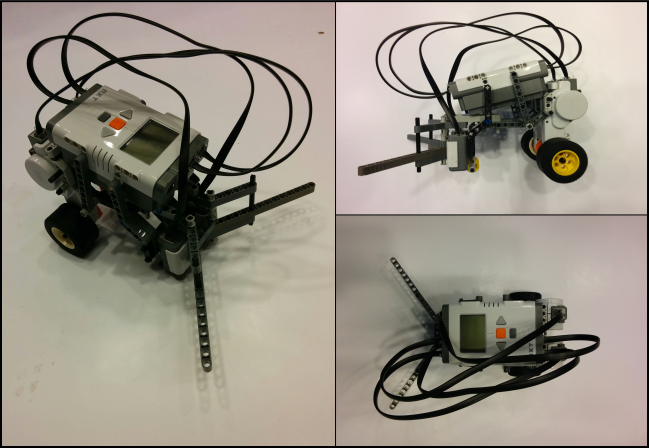
\includegraphics[width=10cm]{Fig1.png}
\centering
\caption{Images of the built robot.}
\label{fig:robotImage}
\end{figure}



\pagebreak
\section{Software Design}
In order to control and stabilize the segway a the communication with the accelerometer/gyroscope must be established.
This must data received must then be processed in order to control the motors according to the segways position.



\begin{figure}[H]
\centering

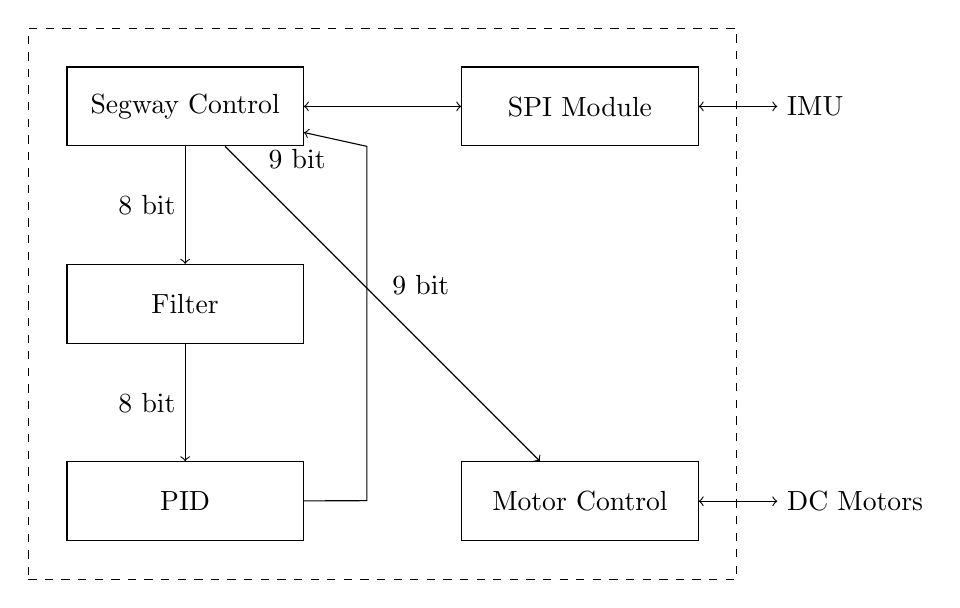
\begin{tikzpicture}[node distance=1cm]
% FPGA border
\node[rectangle,draw,minimum width=9cm, minimum height=7cm, dashed, name=FPGA]  {};

% used to align the insides of FPGA
\node[rectangle,minimum width=5cm, minimum height=5cm, name=FPGAaligne] {};

% components of FPGA
\node[rectangle,draw,minimum width=3cm, minimum height=1cm, name=pid] at (FPGAaligne.-135) {PID};
\node[rectangle,draw,minimum width=3cm, minimum height=1cm, name=communiction] at (FPGAaligne.45) {SPI Module};
\node[rectangle,draw,minimum width=3cm, minimum height=1cm, name=mc] at (FPGAaligne.-45) {Motor Control};
\node[rectangle,draw,minimum width=3cm, minimum height=1cm, name=filter] at (FPGAaligne.180) {Filter};
\node[rectangle,draw,minimum width=3cm, minimum height=1cm, name=segway] at (FPGAaligne.135) {Segway Control};

% nodes outside FPGA
%\node [left=of utos,name=pc] {PC};
\node [right=of communiction,name=spi] {IMU};
%\node [left=of color,name=rgb] {RGB(2:0)};
\node [right=of mc,name=motor] {DC Motors};

% arrows inside FPGA
\draw[<->] (segway) -- node[] {} (communiction) ;
\draw[->] (segway) -- node[left] {8 bit} (filter) ;
\draw[->] (filter) --  node[left] {8 bit} (pid) ;
\draw[->] (segway) -- node[above right] {9 bit} (mc) ;
\draw[->] (pid) --(-0.2,-2.5)--(-0.2,2)-- node[below left] {9 bit} (segway) ;
 
% arrows connected to the outside of FPGA
\draw[<->] (spi) -- node[] {} (communiction) ;
\draw[<->] (mc) -- node[] {} (motor) ;
%\draw[->] (adc) to[out=180, in=0] node[] {} (ad) ;
%\draw[->] (color) to[out=180, in=0] node[] {} (rgb) ;
%\draw[->] (mc) to[out=0, in=180] node[] {} (servo) ;
\end{tikzpicture}

\caption{Block design of the FPGA.}
\label{fig:fpga_sof_design}
\end{figure}


The designed system is comprised by the modules seen in figure \ref{fig:fpga_sof_design}.
Here the \textit{Segway Control} block is the main part of the system, used to combine the different components into one.
The \textit{SPI Module} takes care of the communication with the accelerometer and gyroscope by sending data to such when asked for by the \textit{Segway Control} module.

Data from such is then send to the \textit{Filter} to predict an angle.
From here the angle is passed to the \textit{PID} in order to generate a duty cycle which is then passed back to the main module, the \textit{Segway Control}.
The \textit{Segway Control} hence also takes care to set the right ports on the H-bridges, through the \textit{Motor Control} unit, depending on the speed and direction bit generated by the \textit{PID}.
The five components are explained further throughout this section.


\subsection{Graph Structure}
The graph is used to store the possible route to the solution of the sokoban problem.
It consist of a set of nodes representing states in the solution.
The nodes link to each other depending on the possible ways in which one state can be reached from another.

A state in the sokoban problem can be represented in many ways.
In this implementation it was chosen to have a new state for each diamond push.
The extra cost of going from one state to another, is then the number of steps the robot has to take, in order to reach the new state.
In this way, only the points of interest is stored in the graph, that is the points where the diamonds move and where on the map the robot is standing after the move.
On of the necessary data elements in each node, apart from the cost, is then the shortest path of executing the change of state in terms of moves in the directions north, south, east and west.



\subsection{Heuristics Calculation}
In order to boost the algorithms performance a heuristic is used to make it an A* algorithm.
In order to have a valid A* algorithm, this heuristic should be equal to or less than the actual cost to reach the goal.
This would then ensure that the shortest path, in terms of robot moves, is found as the first path by the algorithm.

A good heuristic is a heuristic that comes as close to the actual distance to the goal as possible.
A heuristic should hence be found to estimate the cost as accurately as possible, but without taking to much computational effort, since it has to be executed for every node created.

The Manhattan distance is a fairly obvious chose for a heuristic when regarded that the robot is only 4-connected.
The disadvantage of using this algorithm is, however, that it does not take the obstacles into account when calculated.
This gives a heuristic which is in many cases much smaller than the actual cost to reach the goal.
A cost taking the walls into account was therefore devised.
Instead of taking the Manhattan distance from every object to the nearest goal on the map, the path from every possible spot on the map to the nearest goal can be precomputed taking the walls into account.
The distance from a point in the 2D space to the nearest goal is then stored in a map such that the cost of bringing every diamond the nearest goal is found in constant time.
In order to find this cost a map is used where only the goals and walls are indicated.
A wavefront originating in all the goals is then spread out across the map simultaneously such that all the reachable positions on the map are assigned their respective cost.
The result of such a process is seen in figure \ref{fig:orig_testmap} and \ref{fig:orig_costmap} where they are the original (empty) map and the updated map with the cost for every position in the map respectively.


\begin{table}[H]
\begin{subtable}{.5\linewidth}
\centering
\begin{tabular}{| *{8}{c} |}
\hline
X & X & X & X & X & X & X & X \\
X & X &   & X & X &   &   & X \\
X &   &   &   &   &   &   & X \\
X & G & X &   &   &   &   & X \\
X & G & X &   & X & X &   & X \\
X &   &   &   &   & G &   & X \\
X &   &   & G &   &   & G & X \\
X & X & X & X & X & X & X & X \\
\hline
\end{tabular}
\caption{Original test map.}
\label{fig:orig_testmap}
\end{subtable}
%
\begin{subtable}{.5\linewidth}
\centering
\begin{tabular}{| *{8}{c} |}
\hline
X & X & X & X & X & X & X & X \\
X & X & 3 & X & X & 6 & 5 & X \\
X & 1 & 2 & 3 & 4 & 5 & 4 & X \\
X & 0 & X & 3 & 4 & 4 & 3 & X \\
X & 0 & X & 2 & X & X & 2 & X \\
X & 1 & 2 & 1 & 1 & 0 & 1 & X \\
X & 2 & 1 & 0 & 1 & 1 & 0 & X \\
X & X & X & X & X & X & X & X \\
\hline
\end{tabular}
\caption{Cost test map.}
\label{fig:orig_costmap}
\end{subtable}
\caption{Result of using the proposed heuristic calculations on a given map.}
\end{table}


\subsection{Node Validation}
When the graph is constructed a massive amount of nodes in the possible direction towards the goal are added to the graph.
This does however also require care in order to validate the nodes before they are added to the closed list in order to prevent excessive memory and time consumption.

Each node must hence be tested in the search for the solution in order to prevent duplicates using all the system memory and processing time.
In order to reduce the check uptime when validating a specific state, it was chosen to use a hash-table to validate if a node is present in the closed-set.
For this to work a hashing value for each node is generated.
This is done using the coordinates of the diamonds and the robot at each state.
The position of such was hence combined into a string where the sorted diamonds position is added to the string first and then followed up with the position of the robot.
This is then used as the unique key in the hashing table preventing the table from being filled with duplicates.

When solving the Sokoban problem furthermore a check for validity of the state is performed.
This is done by considering if any of the diamonds has gone into a deadlock.
Since there are many different deadlock situations, it was chosen only to implement the most simple deadlock arising when pushing a diamond into a corner that is not a goal.
This prevents some of the paths explored being invalid because once gone into a deadlock is entered, the goal is not obtainable from the specific path.
Furthermore a deadlock detection is able to reduce the graph and hence improve the time taken to find the solution on maps where many deadlocks can be entered.


\todo[inline]{implement deadlock as a map for lookup? and then include more deadlock situations?}
\subsection{Path Converter}
Once a path to the sokoban problem is found, it must be translated into something understandable by the robot.
Hence a in between layer was created to make this conversation.

This takes a path and converts it from north, south, east and west to forward, backward, left and right.
Where the robot is executing its steps relative to the direction it is currently facing.

This conversion is made taken into account the direction the robot is facing.
Furthermore the robot has to push the diamonds on the map completely to the next position and then back away to its own square when the last of a sequence pushes is completed.
\subsection{System Test}
%The sokoban solver was implemented as an A* algorithm in C++ with focus on memory consumption and processing time.
%In order to test quantify the final program then this is tested in regards of these factors.

%The program was written for single core processing only and executed on a Intel Core i7-3610QM running at 2.3GHz with a total of 8GB RAM running Ubuntu.

The program was first tested on the handed out test map from the competition of year 2014.
This was used to see if the solution found was as short as path supplied and to consider the memory consumption and processing time of the program.

The path found by the program was, like the solution provided, 124 steps indicating that the solver is capable of returning the right result.
The memory used by the program is seen in figure \ref{fig:memoryconsumption2014}.


As seen on figure \ref{fig:memoryconsumption2014}, then the memory consumption is just below 30MB.
Where the main memory consumption is from the openlist (red), the strings used for hashing (yellow), and the closed list (green).

The solver was furthermore tested on a set of different microban maps to see if the program works and this was confirmed.
Theoretically the solver can solve any map, as long as it has enough time and memory to do so.


\begin{figure}[H]
\centering
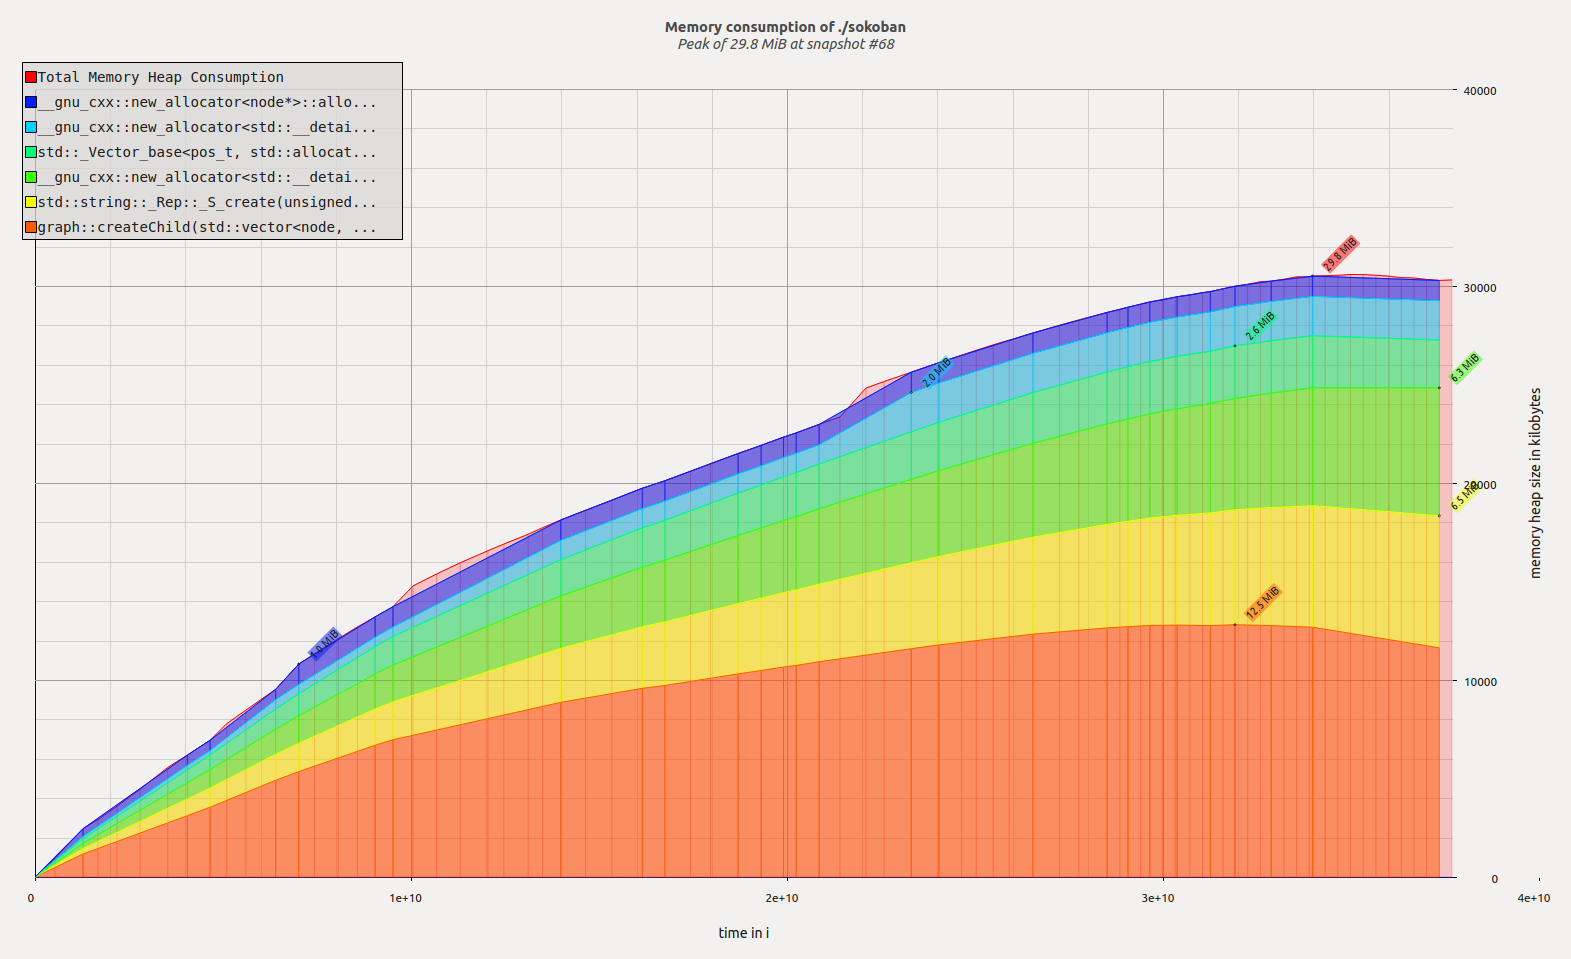
\includegraphics[width = 0.8 \linewidth]{graphics/memoryconsumption.png}
\caption{Memory consumption of the program when computing the solution for the competition of year 2014.}
\label{fig:memoryconsumption2014}
\end{figure}

In its current version, the map size is however limited to to maps with a total map size less or equal to 255 squares.
This is due to the implementation of the closed list and the choice of hashing value.
%It can however be increased at a cost of more memory used per node in the table.





\subsection{Conclusion}
An A* algorithm was devised to solve the Sokoban problem.
The algorithm uses a graph structure where the nodes represent diamond pushes with the cost being the number of steps the robot must move in order to achieve the state.

The heuristic for the A* algorithm was found calculating the cost for the robot to move each diamond from their current position to the nearest goal.
This technique takes into account the walls on the map, but disregard the diamonds left on the map disrupting the path.
Furthermore the cost of moving in between the diamonds and the fact that one goal may be considered the destination of multiple diamonds is not taken into account using this method.

The nodes in the graph where also validated using their state, in form of the diamonds and robots position, as the key in a hashing table.
Furthermore the states are checked for simple deadlock situations.





\pagebreak
\section{Hardware Tests}

\subsection{Hardware Test}

The functionality of the behaviours implemented can be tested individually.
Nevertheless, a more robust way of testing the behaviours is to combine them in certain test circuits that can be looped to check the reliability of these behaviours.
By building a more complex circuit to test, the different behaviours can be tested in different ways so the position of the robot changes before each of them.

This way, three different experiments have been executed to test the reliability of the robot:

\begin{enumerate}
	\item First, a test to check the robot is able to find, follow and get a good position on a line after right and left turning. 
With this test we can test the follow line, and turning behaviours.
The circuit used in this test was a "8", that means, the robot should turn left 4 times and then right 4 times in a row
.

	\item The second test executed has looked at the ability of the robot to go back in a intersection and turn to different directions after finding the previous intersection.
This test has been done running a circuit where the robot goes back, find the next intersection and goes back to the previous one. 
Then the robot turns in different directions each time, checking the response of all of them in different cases, as these directions are mixed.

	\item Finally, a experiment with a can has been executed to test the robot hability to push and place correctly the can.
In this experiment, the robot has to use all the different behaviours to move the can from one position to another and then to the original position again.

\end{enumerate}

The circuits used in each experiments are shown in the figure \ref{fig:testMaps}

Each of the three experiments have been executed starting with a full power battery and the circuit set for each one has been repeated 20 times in up to 10 trials without a battery change or charge.
The time needed to complete the 20 laps has been measured for each trial.
This allows us to determine too the fucionality and response of the robot in long runs.

About the light sensors, they have been tested to measure their response to different ambient light levels and the efectivity of shielding these sensors has been proved.
The information about this research is attached in \_reftolightsensors.


\begin{figure}[H]
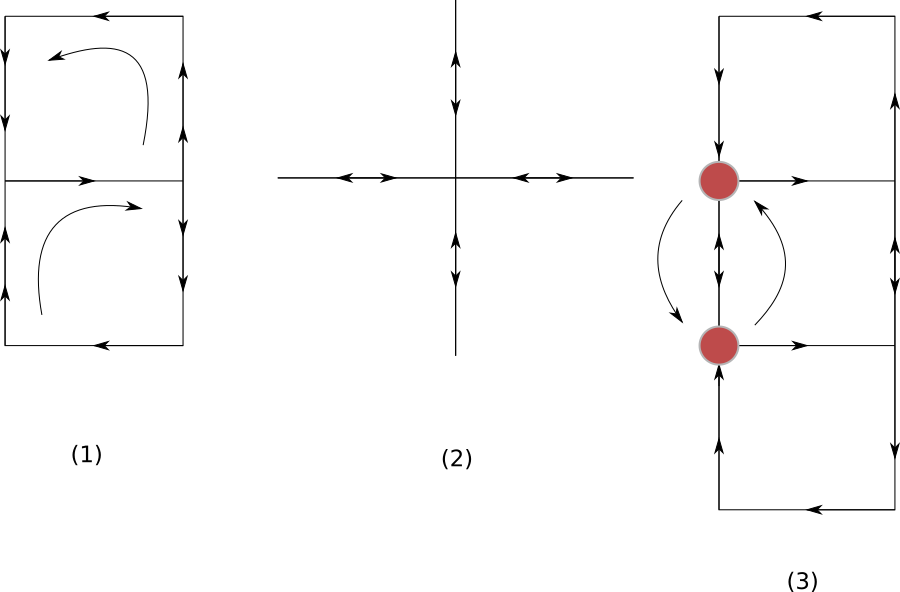
\includegraphics[width=10cm]{Test_circuits.png}
\centering
\caption{Scheme of the circuits used in the tests. 1, loop for turning behaviours. 2, used for pushing and going back behaviours. 3, used for testing the pushing behaviour with a can. }
\label{fig:testMaps}
\end{figure}


\subsection{Results}
	The results of the tests shown in table \ref{tab:Experiment1} allow to conclude that the chosen configuration is robust enough to complete any sokoban map.
	All the behaviours have been tested and have worked in the most of the cases, but they failed a couple of times probably because a low battery problem, as the failures start when the robot has been running for a long time.
	This has happened in the pushing and going back behaviour concretely, what means it is the weakest part of the implementation.
	Nevertheless, the number of failures of this behaviour is small enough to ignore them.
	
	As the time spent running without battery charge has been above the 30 minutes in all experiments, it can be assumed that the robot will not have power problems during it's operating time, which is of 15 minutes as maximum during a race.
	Also it can be seen that the different robot behaviours are strong enough to be successfully executed in most of the times, but is not perfect, as can be seen in some failed tests.
	
	Finally, it is possible to say that the robot configuration is robust under different light levels thanks to the used shield, and also can be said that the robot control is able to complete its task.


\begin{table}[H]
	\center
	
	\begin{tabular}{|l|c|r|c|r|c|r|}
	  	\cline{2-7}
	  	\multicolumn{1}{r}{}
 		&  \multicolumn{2}{|c|}{Map 1}
 		& \multicolumn{2}{|c|}{Map 2} 
 		& \multicolumn{2}{|c|}{Map 3}  
		 \\ \cline{2-7}
		\hline
		Run & Success & Time & Success & Time & Success & time \\
		\hline
		1 	& Yes & 6'26'' & Yes & 5'28'' & Yes & 8'16''\\
		2 	& Yes & 6'21'' & Yes & 5'33'' & Yes & 8'15''\\
		3 	& Yes & 6'27'' & Yes & 5'29'' & Yes & 8'17''\\
		4 	& Yes & 6'29'' & Yes & 5'30'' & Yes & 8'05''\\
		5 	& Yes & 6'33'' & Yes & 5'31'' & Yes & 8'15''\\
		6 	& Yes & 6'33'' & No  & 5'10'' & Yes & 8'10''\\
		7 	& Yes & 6'55'' & Yes & 5'34'' & Yes & 8'25''\\
		8 	& Yes & 6'52'' & Yes & 5'41'' & Yes & 8'54''\\
		9 	& No & LOWBAT  & No  & 1'13'' & No 	& LOWBAT\\
		10 	& No & LOWBAT  & No  & 1'50'' & No 	& LOWBAT\\		
		\hline
	\end{tabular}

	\caption{Table of results for the experiments. It is shown for each experiment and result the success or failure of the test and the time expended on it. In the case of the failed trials, the time shown represents the moment when the robot was lost. The LOWBAT statement means the robot finished his power and the experiment finished.}
	\label{tab:Experiment1}
\end{table}

\pagebreak
\section{Conclusion}





\end{document}